\section{Model 3}


The results displayed in this section are for the uncertainty involved
in the calculation of flamespeed depending on two parameters: the
activation energy for the fall off reaction in the ozone mechanism and
the pre exponential factor for third reaction in the mechanism. The
percentage of ozone is taken as 40, 46, 53, 75, and 100 percent
according to the experimental data available to us from
Streng\cite{Streng}.
%% In the figure~\ref{subfig-m3-KDE-A3} and
%% figure~\ref{subfig-m3-KDE-E3}, we display results for sample
%% size 1e7 and surrogate of 100X100 points.  We show the the KDE for
%% parameters log($A_3$) and $E_3$.


Figure~\ref{subfig-m3-samp-A3} and
Figure~\ref{subfig-m3-samp-E3} show posterior distributions, for a constant surrogate size of
$100\times 100$, with varying number of MCMC samples from 1e5 to
1e7. Convergence is observed.
%% The plot is done for raw chain size of $1e7$,
%% $2e7$ , $5e7$, and $9e7$ is taken.
Figure~\ref{subfig-m3-surr-A3}
and Figure~\ref{subfig-m3-surr-E3} show a convergence
study for surrogates with differing number of interpolation
points. As we increase the number of points in the surrogate, we
observe convergence in the posterior KDEs. Results are shown for
surrogate sizes ranging from $75\times 75$ to $200\times 200$ for both
 $\log(A_3)$ and $E_3$; the MCMC chain
size is $1e7$.
%% For different starting points of MCMC chain, the MAP
%% point of the resulting pdf does not change. The surrogates for
%% individual concentrations are constructed using linear interpolation
%% function. The initial guess for the MAP point is calculated using
%% Nelder Mead optimization technique.


Figure~\ref{subfig-m3-1:mean_3} and
Figure~\ref{subfig-m3-2:autocr_3} show mean and autocorrelation
for the samples of the parameters $\log(A_3)$ and $E_3$ in order to assess
the required chain thinning.
%% The mean plot
%% shows the initial instability due to sum in period of MCMC and after
%% that it remains constant. It shows us that we should be using at least
%% more than these number of samples for our analysis.
Figure~\ref{subfig-m3-1:a3_distribution} and
Figure~\ref{subfig-m3-1:e3_distribution_3}
shows the posterior of $\log(A_3)$ and $E_3$, respectively, using the
final thinned MCMC chain. The $\log(A_3)$ posterior has the following
statistical moments: Mean: 32.86, Std. Dev.: 0.97, Skewness: -0.96, and
Kurtosis: 1.79.  The $E_3$ posterior has the following statistical
moments:
Mean: 57.50, Std. Dev.: 8.36, Skewness: -0.77, and
Kurtosis: 1.20.


 It is necessary to ensure that the samples of the parameter which we
 are drawing are fitting the flamespeed values of the
 experiment. Figure~\ref{subfig-m3-1:40_3} through
 Figure~\ref{subfig-m3-5:100_3},
 illustrate the calculated flamespeed
 using the generated surrogate models for all the
 parameter samples drawn from the final posterior distribution for
 each parameter.




 %% \begin{figure}[H]
%%    \centering
%%    \subfloat[KDE \label{subfig-m3-KDE-A3}]{
%%      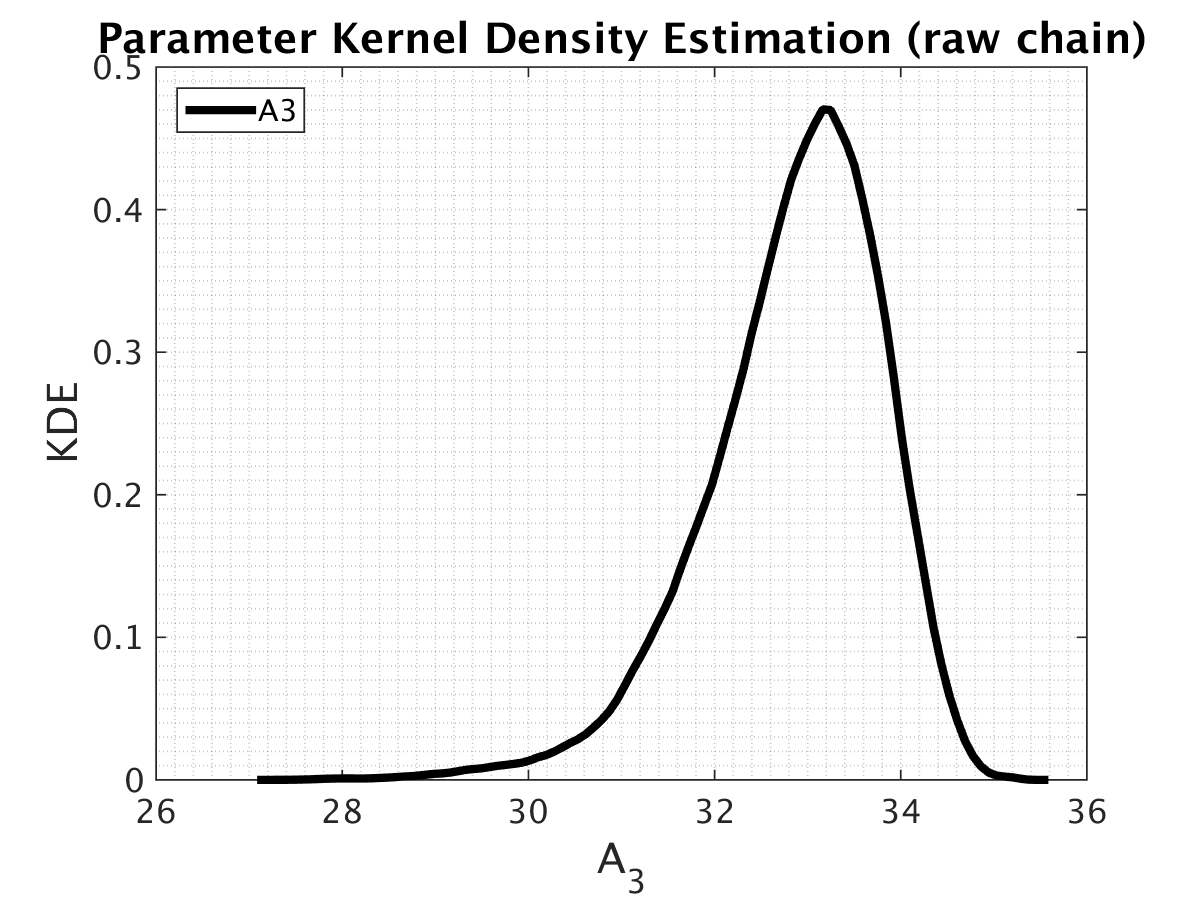
\includegraphics[width=0.45\textwidth]{model_3/kde_1} }
%%    \subfloat[KDE \label{subfig-m3-KDE-E3}]{
%%      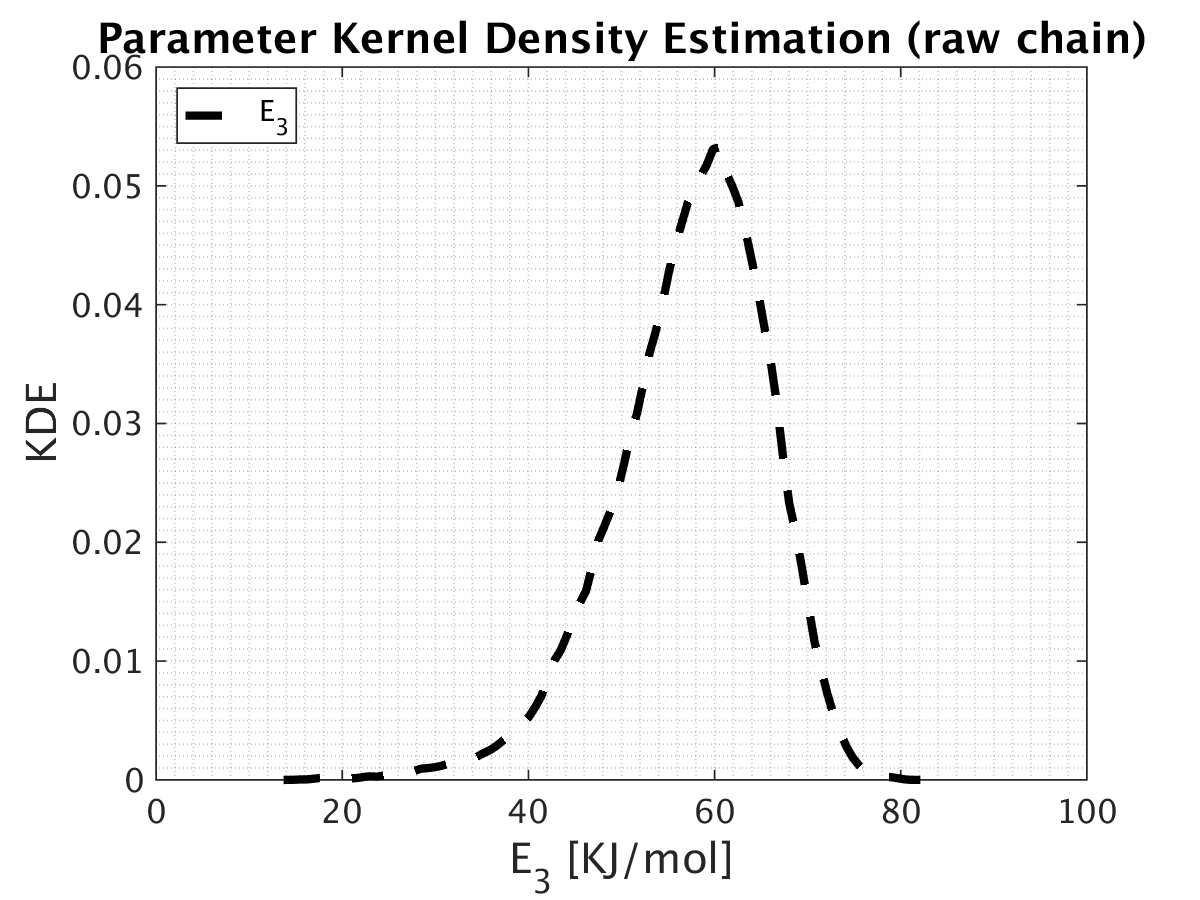
\includegraphics[width=0.45\textwidth]{model_3/kde_2} }
%%     \caption{Results for sample size 1e7}
%% \end{figure}

 \begin{figure}[H]
   \centering
   \subfloat[log($A_3$) sample convergence \label{subfig-m3-samp-A3}]{
     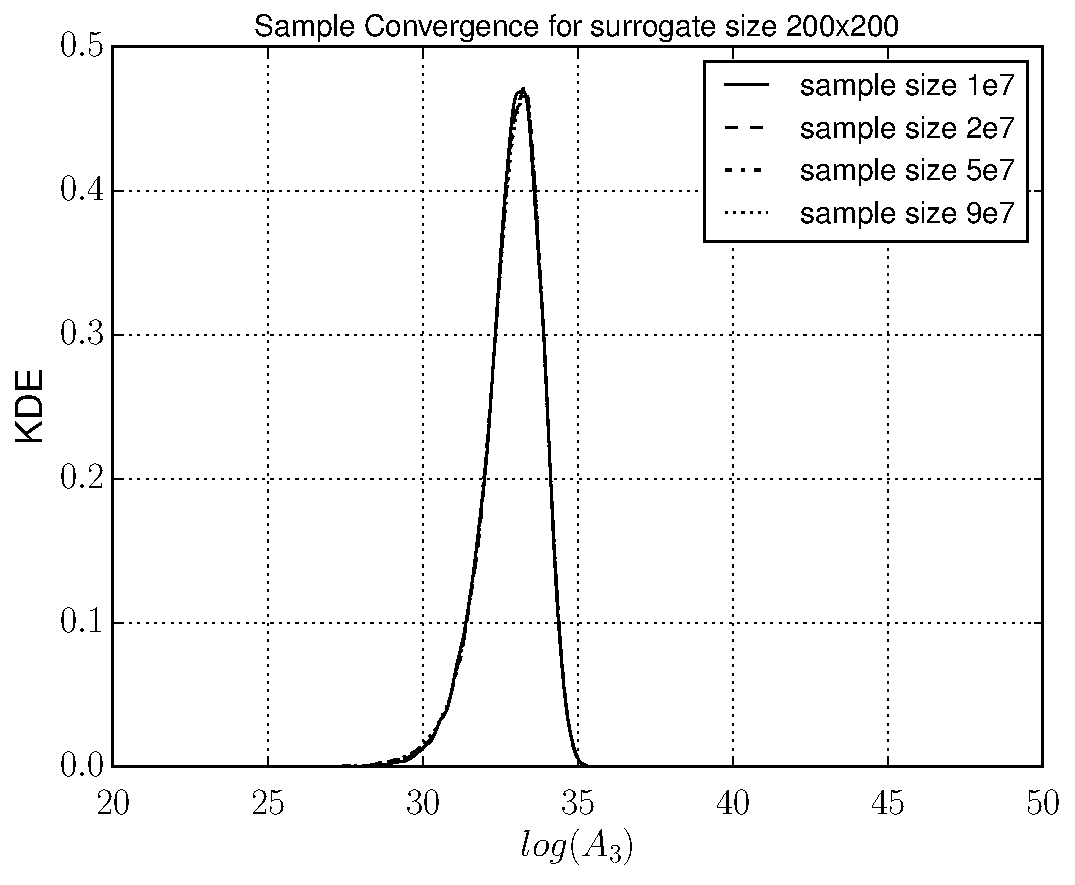
\includegraphics[width=0.45\textwidth]{model_3/sample_conv_A3.pdf}
   }
   \subfloat[$E_3$ sample convergence \label{subfig-m3-samp-E3}]{
     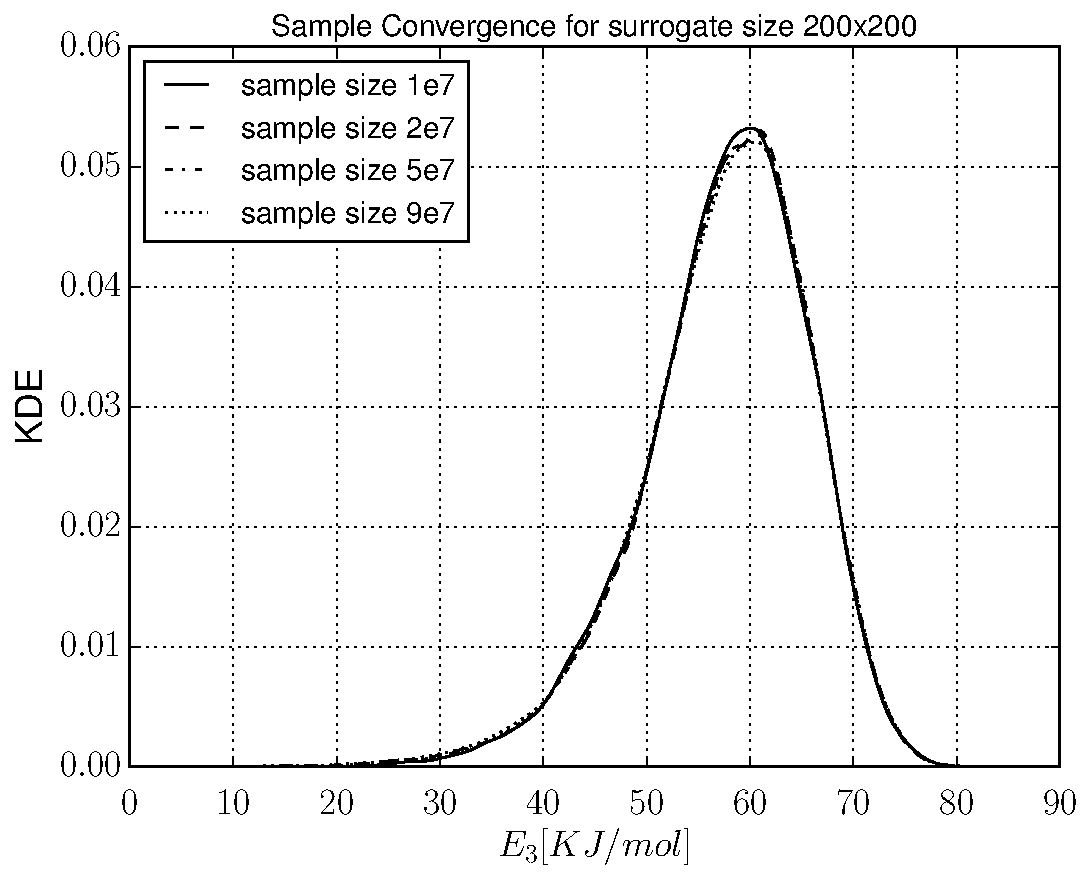
\includegraphics[width=0.45\textwidth]{model_3/sample_conv_E3.pdf}
   }
    \caption{Convergence assessment with respect to increasing
              number of MCMC samples for $\log(A_3)$ and $E_3$.}
\end{figure}

 \begin{figure}[H]
   \centering
   \subfloat[log($A_3$) surrogate convergence. \label{subfig-m3-surr-A3}]{
     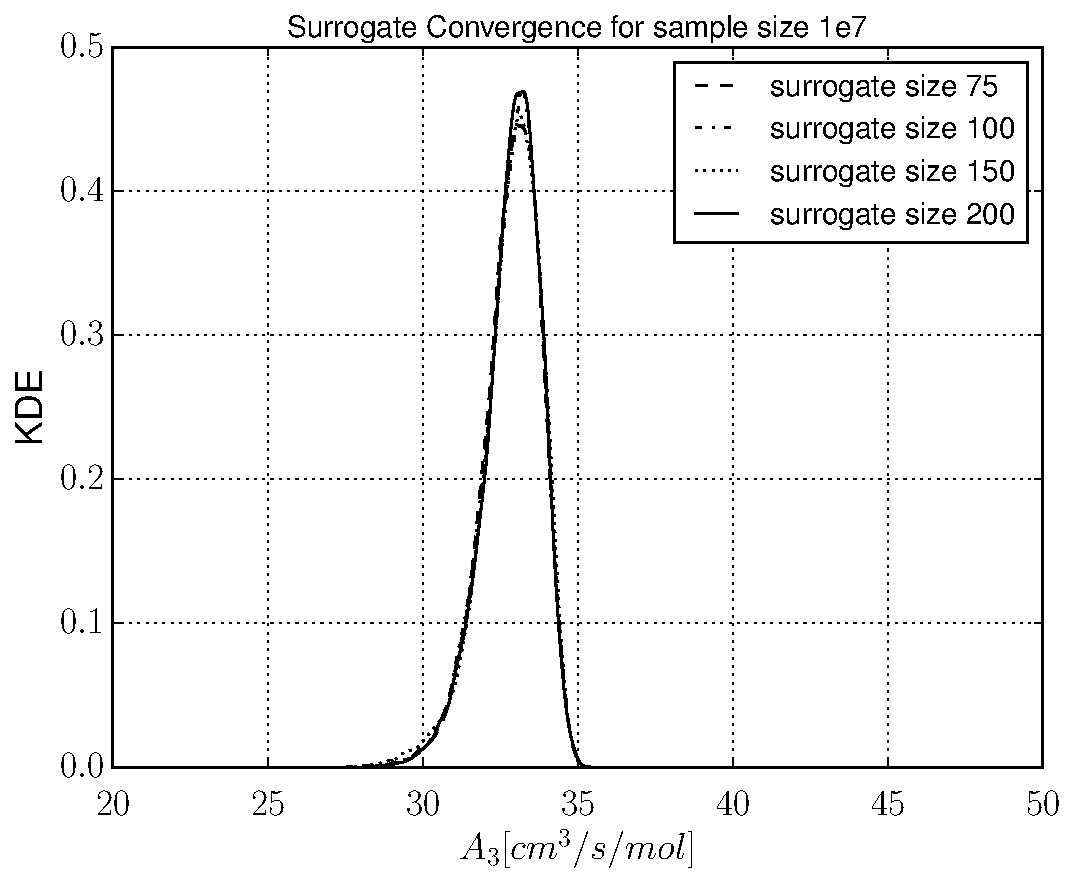
\includegraphics[width=0.45\textwidth]{model_3/surrogate_conv_A3.pdf}
   }
   \subfloat[$E_3$ surrogate convergence. \label{subfig-m3-surr-E3}]{
     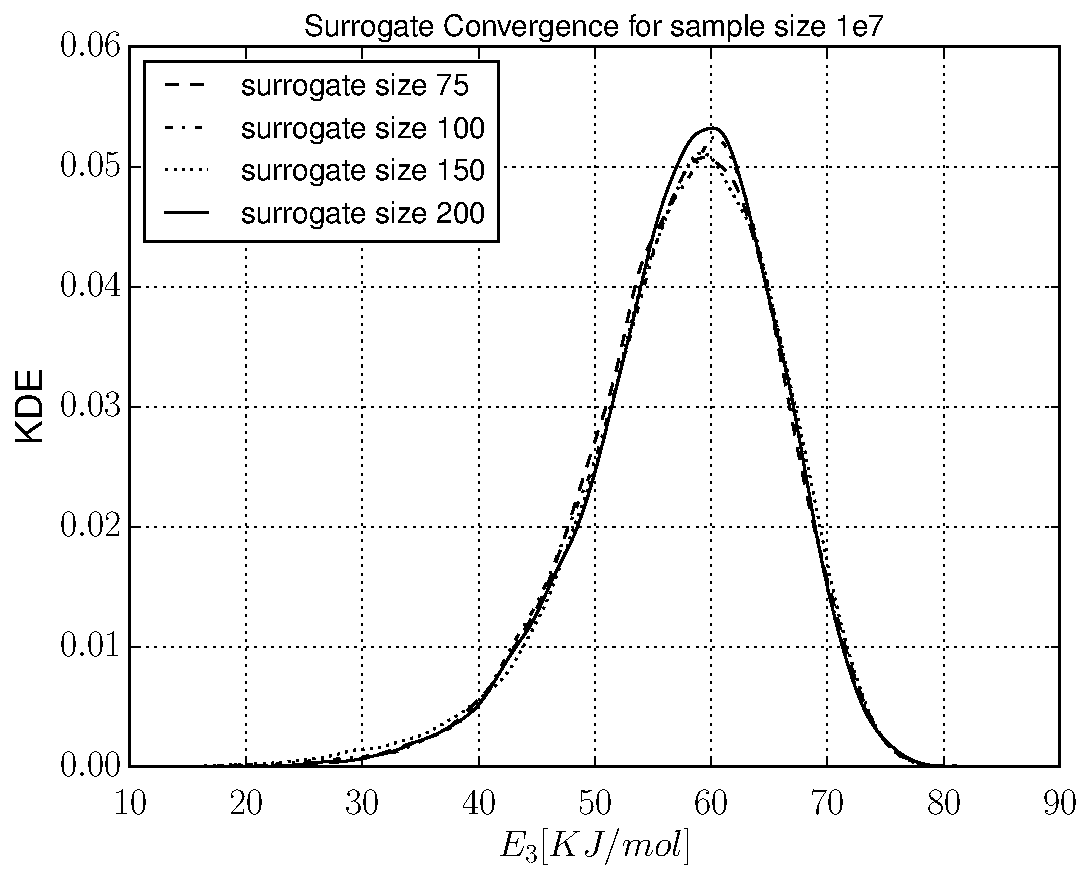
\includegraphics[width=0.45\textwidth]{model_3/surrogate_conv_E3.pdf}
   }
   \caption{Convergence with respect to increasing number of
     surrogate evaluations points for $\log(A_3)$ and $E_3$.}
\end{figure}

 \begin{figure}[H]
   \centering
   \subfloat[ Mean \label{subfig-m3-1:mean_3}]{
     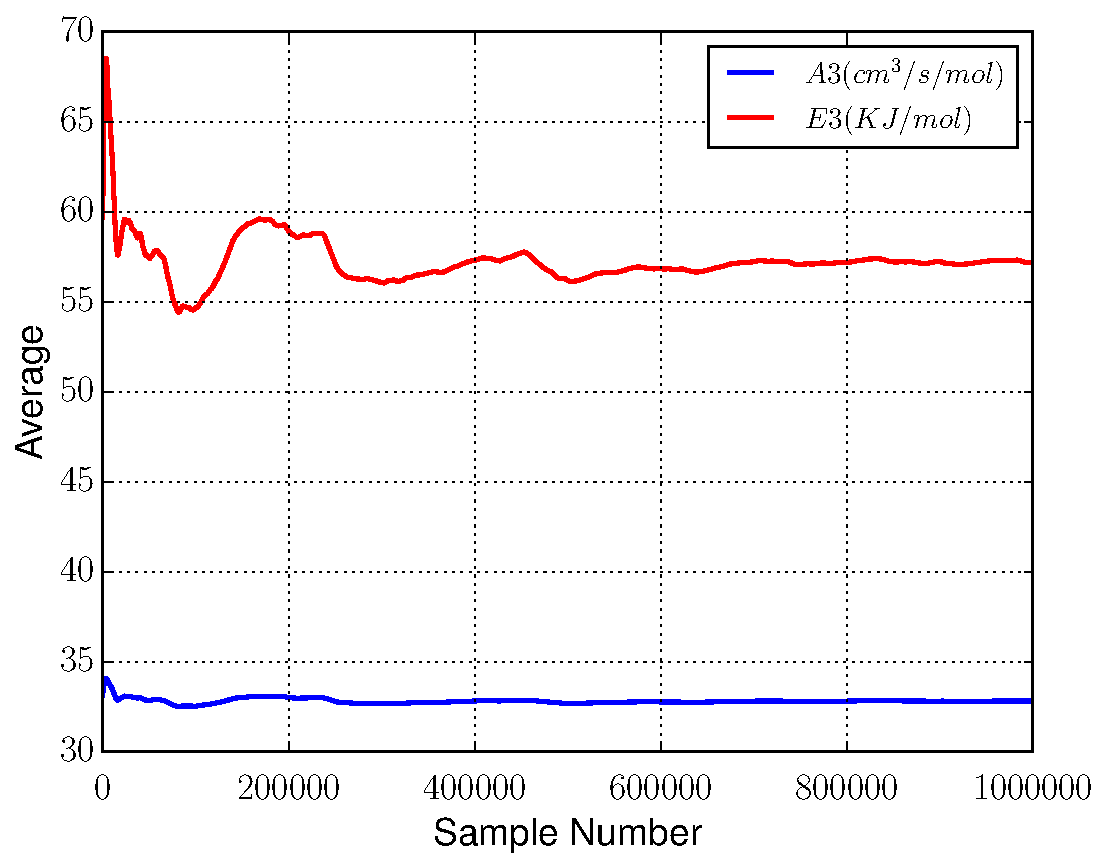
\includegraphics[width=0.45\textwidth]{model_3/M1_running_avg.pdf} }
   \subfloat[Autocorrelation \label{subfig-m3-2:autocr_3}]{
     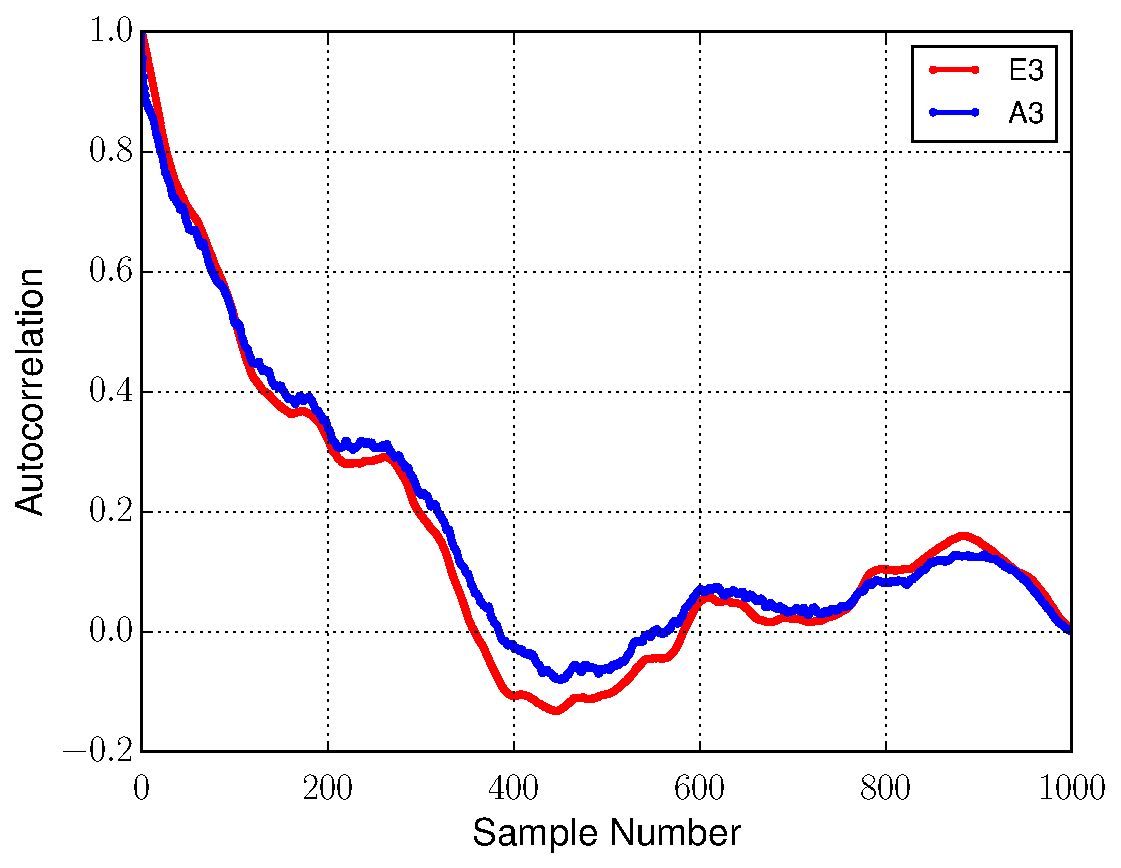
\includegraphics[width=0.45\textwidth]{model_3/M1_autocorr.pdf} }
            \caption{Mean and autocorrelation of unthinned MCMC chain.}
\end{figure}

 \begin{figure}[H]
   \centering
\subfloat[ $E_3$ distribution \label{subfig-m3-1:e3_distribution_3}]{
  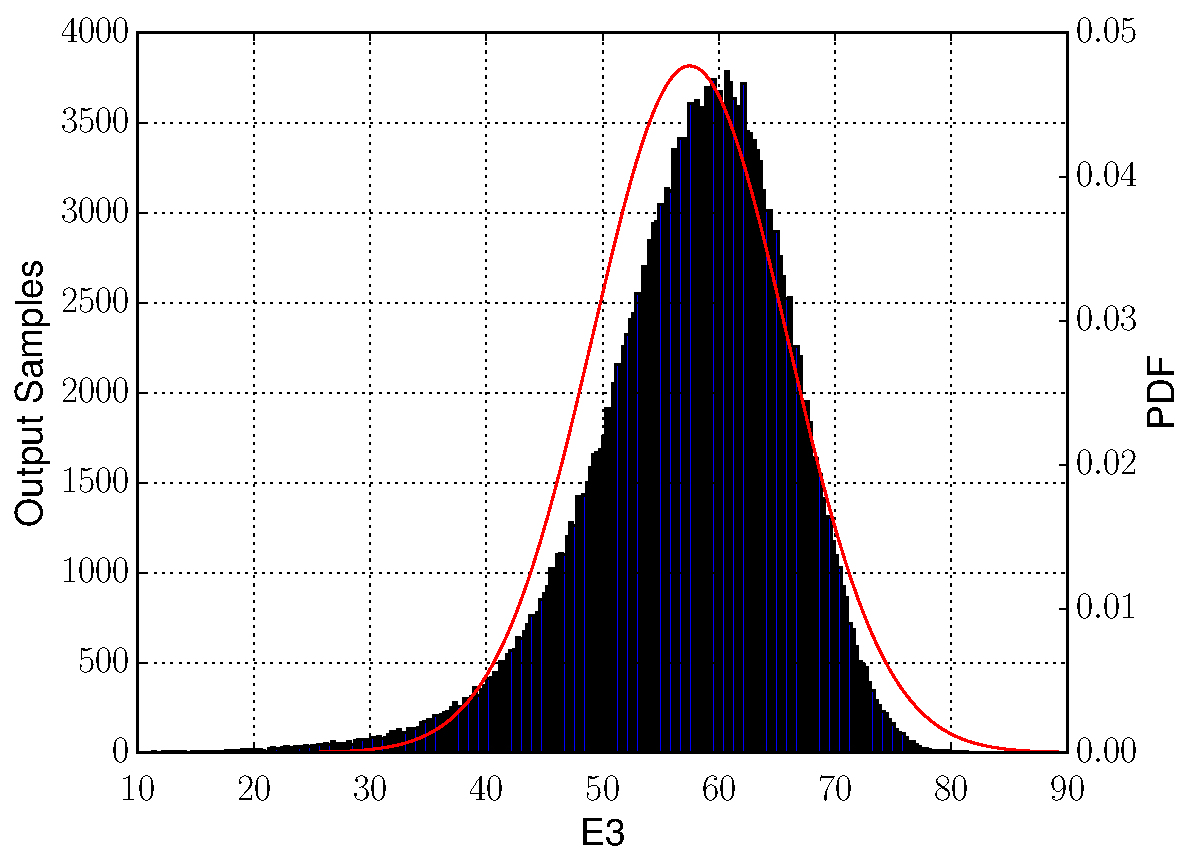
\includegraphics[width=0.45\textwidth]{model_3/E3.pdf} } \subfloat[ log($A_3$)
  distribution \label{subfig-m3-1:a3_distribution}]{
  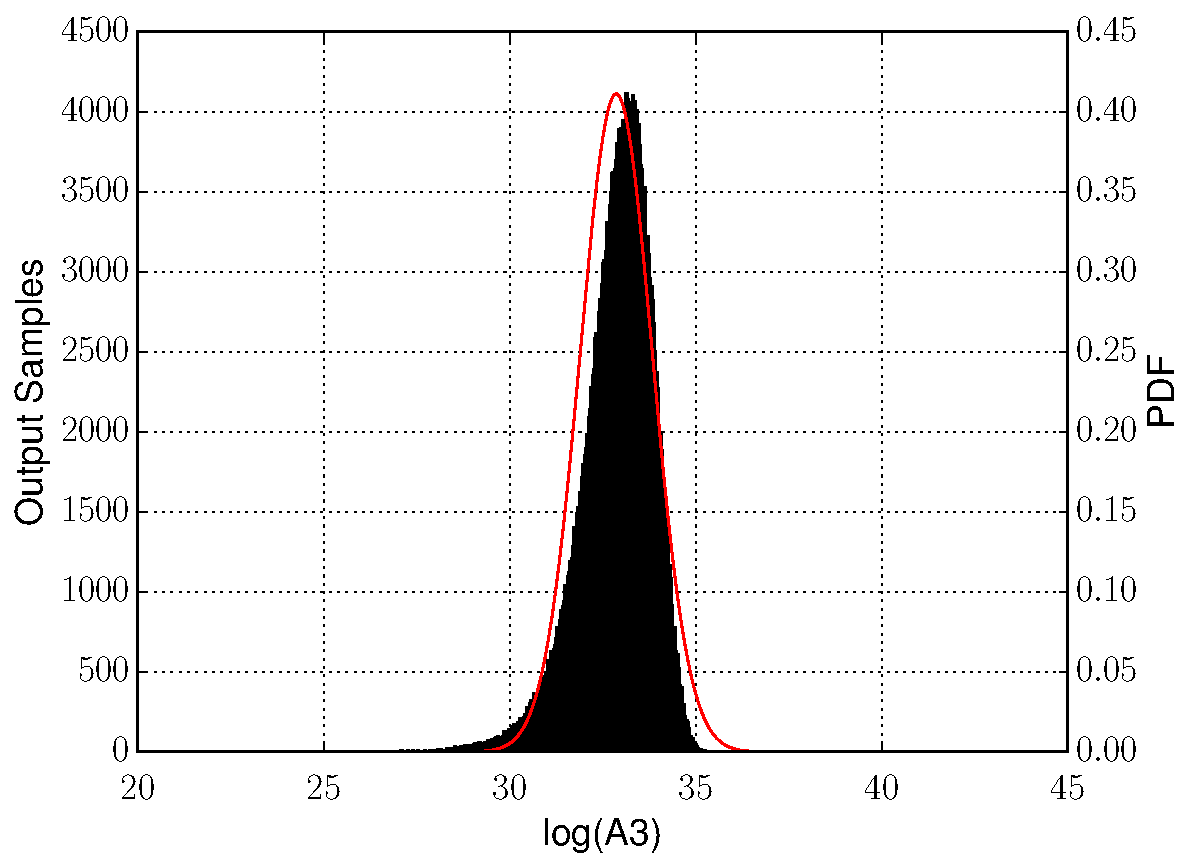
\includegraphics[width=0.45\textwidth]{model_3/A3.pdf} }
            \caption{Thinned $E_3$ and log($A_3$) posterior distributions.}
\end{figure}

 \begin{figure}[H]
   \centering
   \subfloat[ Flame speed for 40 \% ozone. \label{subfig-m3-1:40_3}]{
     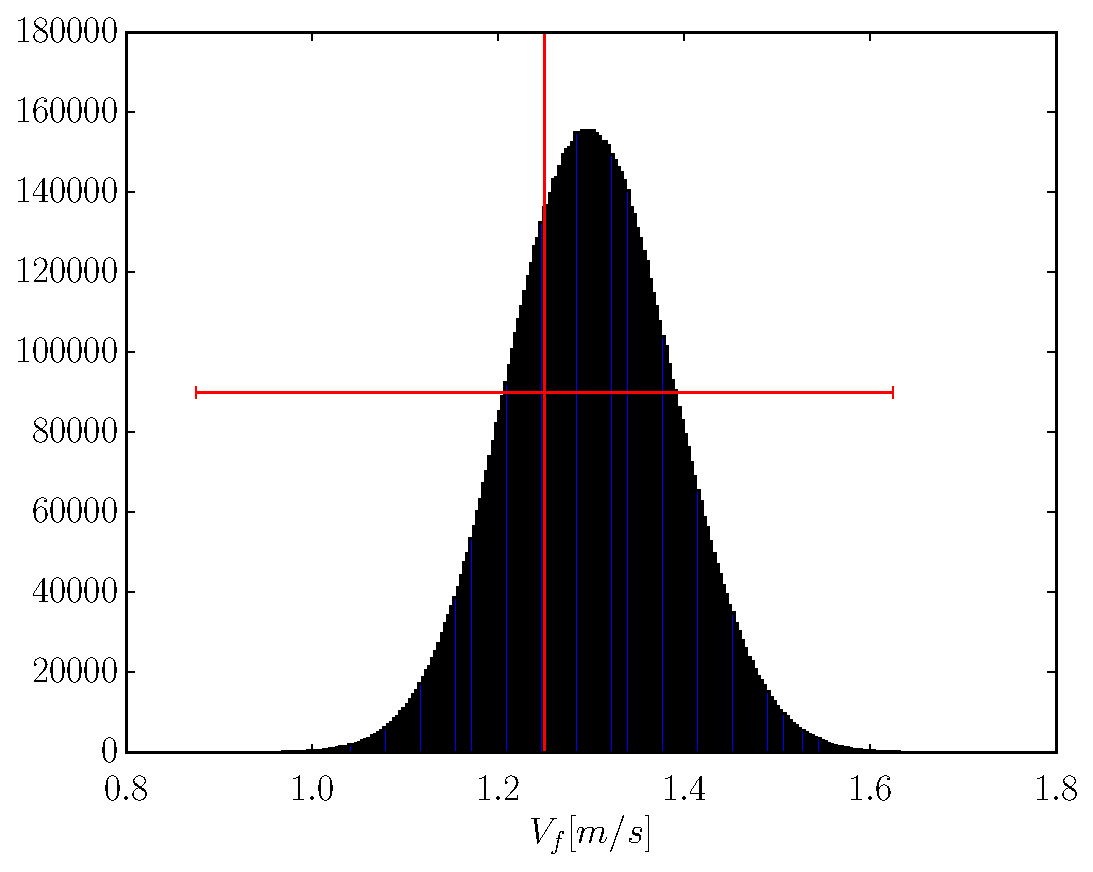
\includegraphics[width=0.45\textwidth]{model_3/flame_40.pdf} }
   \subfloat[Flame speed for 46 \% ozone. \label{subfig-m3-2:46_3}]{
     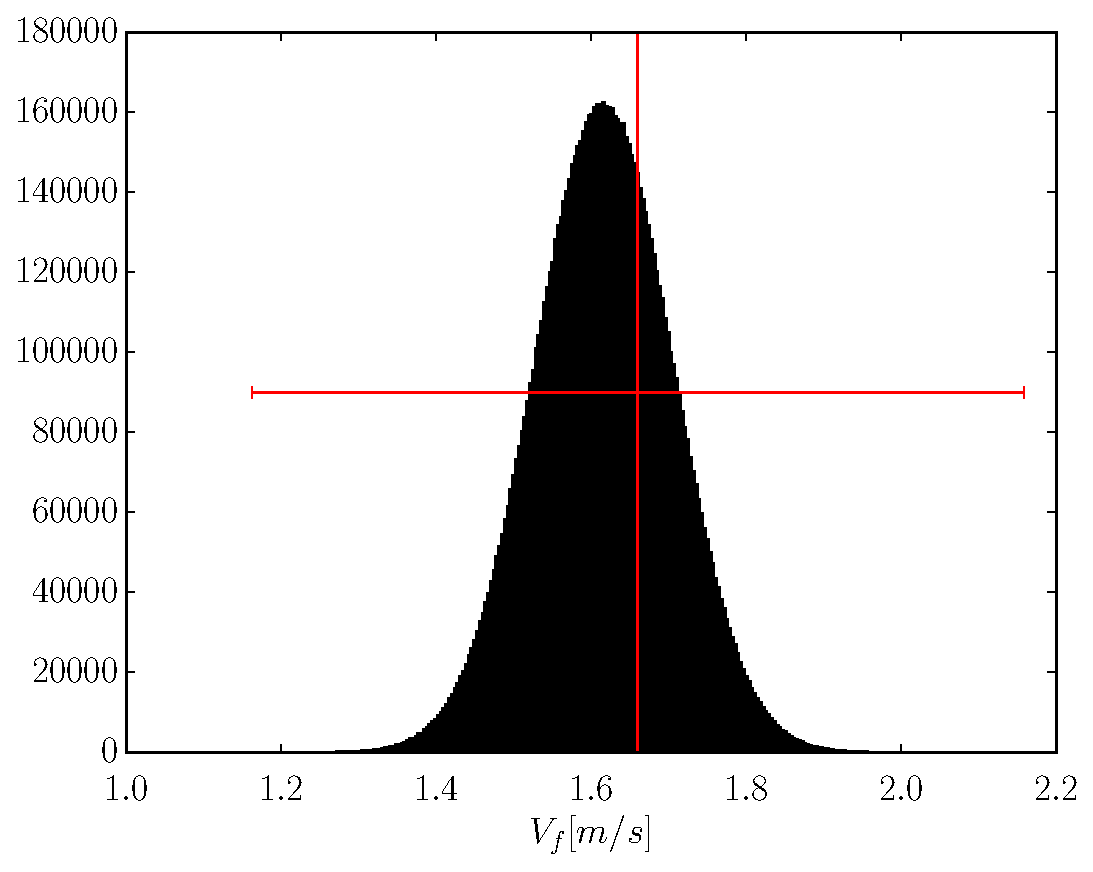
\includegraphics[width=0.45\textwidth]{model_3/flame_46.pdf} }

   \subfloat[ Flame speed for 53 \% ozone. \label{subfig-m3-3:53_3}]{
    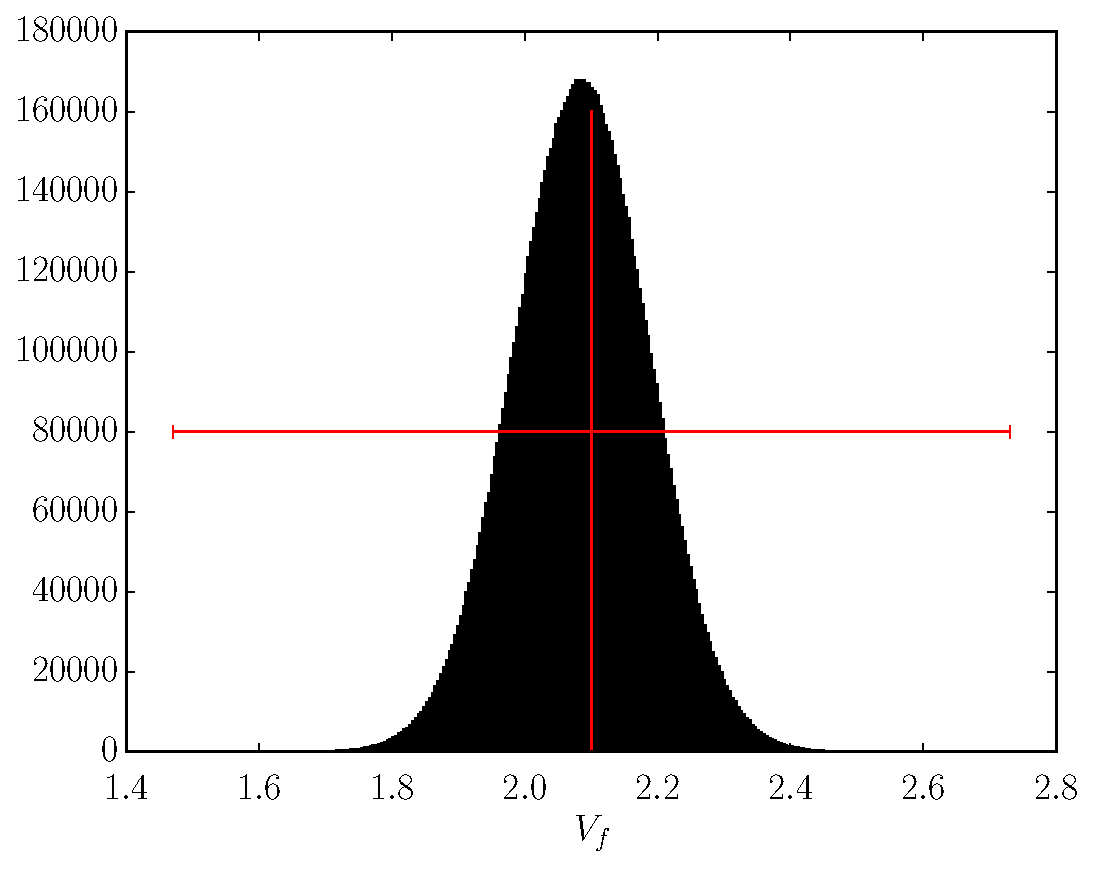
\includegraphics[width=0.45\textwidth]{model_3/flame_53.pdf} }
  \subfloat[Flame speed for 75 \% ozone. \label{subfig-m3-4:75_3}]{
    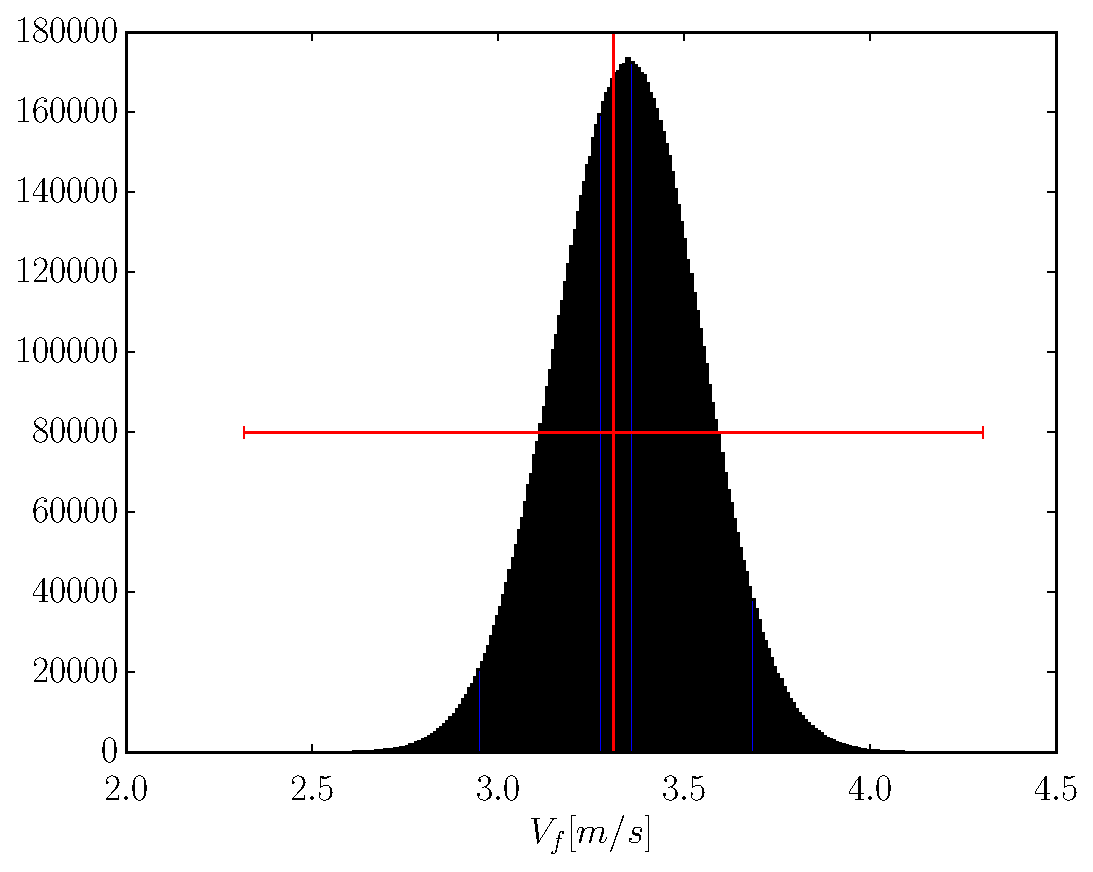
\includegraphics[width=0.45\textwidth]{model_3/flame_75.pdf} }

  \subfloat[ Flame speed for 100 \% ozone. \label{subfig-m3-5:100_3}]{
    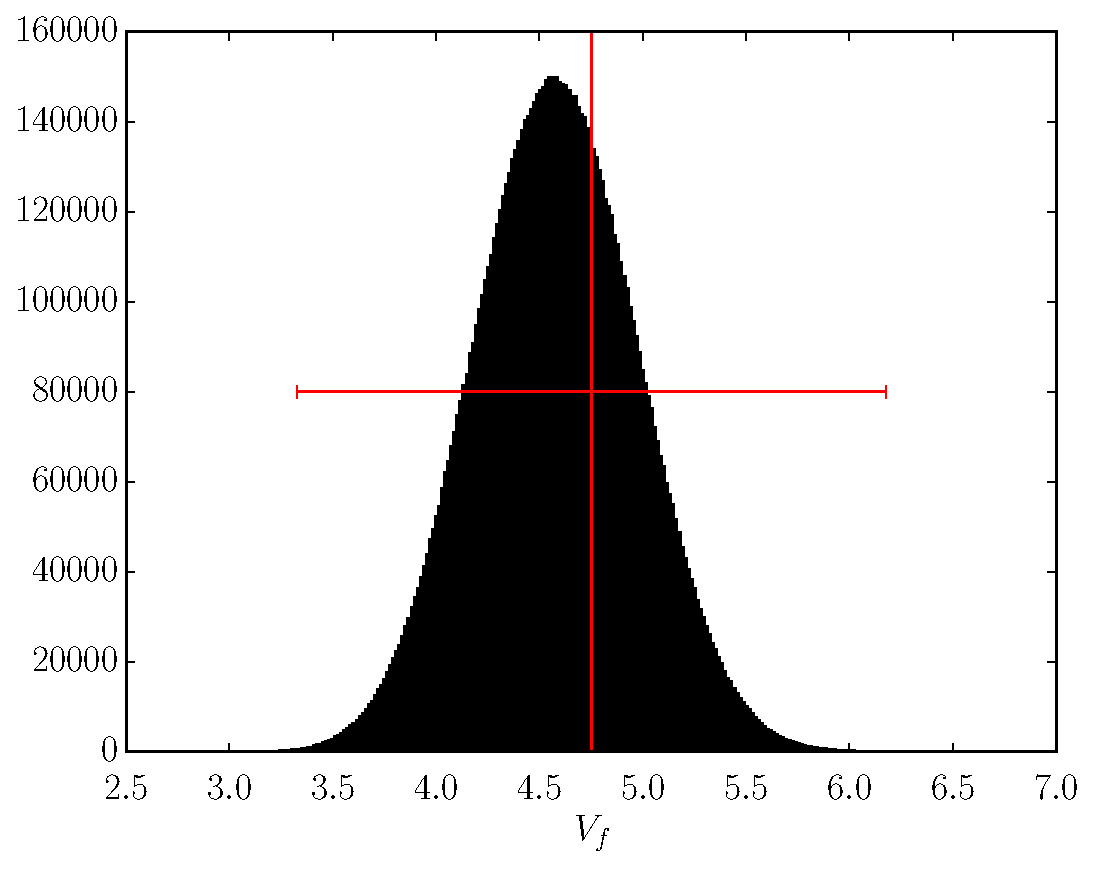
\includegraphics[width=0.45\textwidth]{model_3/flame_100.pdf} }
  \caption{Distribution of flamespeed from $\log A_3$ and $E_3$
    posteriors in order to
     assess quality of parameter fit with experimental data. Red
     vertical line is the data value while the horizontal red line is
     $\pm 30\%$.}
\end{figure}
